\documentclass{article}
\usepackage[margin=1in]{geometry}
\usepackage{amsmath,amsthm,amssymb}
\usepackage{bbm,enumerate,mathtools}
\usepackage{tikz,pgfplots}
\usepackage{chessboard}
\usepackage[hidelinks]{hyperref}
\usepackage{multicol} % Problem 35
\usepackage{xstring} % Difficulty command
\usetikzlibrary{shapes.geometric}

\newenvironment{question}{\begin{trivlist}\item[\textbf{Question.}]}{\end{trivlist}}
\newenvironment{note}{\begin{trivlist}\item[\textbf{Note.}]}{\end{trivlist}}
\newenvironment{references}{\begin{trivlist}\item[\textbf{References.}]}{\end{trivlist}}
\newenvironment{related}{\begin{trivlist}\item[\textbf{Related.}]\end{trivlist}\begin{enumerate}}{\end{enumerate}}

\newcommand\score[1]{
\pgfmathsetmacro\pgfxa{#1+1}
\tikzstyle{scorestars}=[
  star,
  star points=5,
  star point ratio=2.25,
  draw,
  inner sep=3pt,
  anchor=outer point 5
]
  \begin{tikzpicture}[baseline]
    \draw[opacity=0] (0,-0.5) rectangle (0,0.2); % Workaround for whitespace at the bottom.
    \foreach \i in {1,...,4} {
      \pgfmathparse{(\i<=#1?"yellow":"gray")}
      \edef\starcolor{\pgfmathresult}
      \draw (\i*4.5ex,0) node[name=star\i,scorestars,fill=\starcolor]  {};
    }
  \end{tikzpicture}
}

\newcommand{\difficulty}[1]{%
  \IfEqCase{#1}{%
      {1}{
        
\begin{tikzpicture}[scale=0.7, baseline=0.9mm]%
          \definecolor{slopegreen}{rgb}{0.0, 0.5, 0.0}%
          \fill[slopegreen] (0.5,0.5) circle (0.5);%
        \end{tikzpicture}%
      }%
      {2}{
        
\begin{tikzpicture}[scale=0.7, baseline=0.9mm]%
          \definecolor{slopeblue}{rgb}{0.0, 0.44, 1.00}
          \fill[slopeblue] (0,0) rectangle (1,1);%
        \end{tikzpicture}%
      }%
      {3}{
\begin{tikzpicture}[scale=0.7, baseline=0.9mm]\fill (0,0.5)--(0.5, 0)--(1,0.5)--(0.5,1)--cycle; \end{tikzpicture}}%
      {4}{
\begin{tikzpicture}[scale=0.7, baseline=0.9mm]\fill (0.25,0)--(0,0.5)--(0.25,1)--(0.5,0.5)--cycle; \fill (0.75,0)--(0.5,0.5)--(0.75,1)--(1,0.5)--cycle;\end{tikzpicture}}%
      % you can add more cases here as desired
  }[\PackageError{difficulty}{Undefined difficulty level: #1}{}]%
}%
\newcommand{\rating}[2]{\difficulty{#1}\\\score{#2}\\}


\begin{document}
\rating{3}{1}
Consider tilings of the $n \times n$ grid up to $D_8$ action where the
tiles are diagonals.
\begin{figure}[!h]
  \centering
  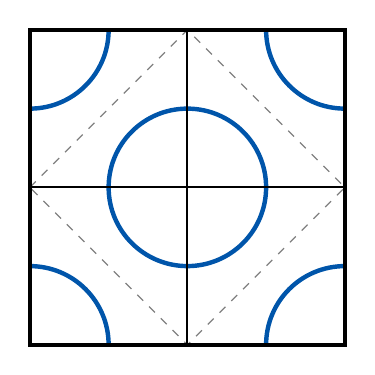
\begin{tikzpicture}[scale=2]
    \draw[ultra thick, draw={rgb:red,0;green,1;blue,2}] 
      (0.5,0) arc (0:90:0.5)    % (0,0)
      (0.5,1) arc (180:270:0.5) % (0,0)
      (2,0.5) arc (90:180:0.5)  % (1,0)
      (1,0.5) arc (270:360:0.5) % (1,0)
      (1,1.5) arc (90:180:0.5)  % (0,1)
      (0,1.5) arc (270:360:0.5) % (0,1)
      (1.5,1) arc (0:90:0.5)    % (1,1)
      (1.5,2) arc (180:270:0.5) % (1,1)
    ;
    \draw[gray, dashed] (0,1)--(1,2)--(2,1)--(1,0)--cycle;
    \draw[ultra thick] (0,0) rectangle (2,2);
    \draw[thick] (1,0)--(1,2) (0,1)--(2,1);
  \end{tikzpicture} \hspace{1cm}
  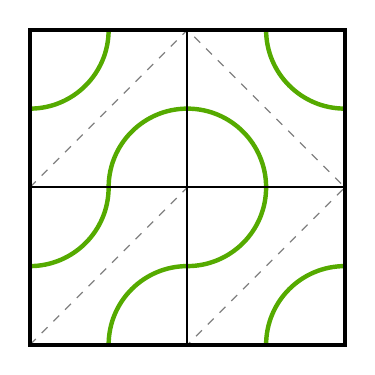
\begin{tikzpicture}[scale=2]
    \draw[ultra thick, draw={rgb:red,1;green,2;blue,0}] 
      (1,0.5) arc (90:180:0.5)  % (0,0)
      (0,0.5) arc (270:360:0.5) % (0,0)
      (2,0.5) arc (90:180:0.5)  % (1,0)
      (1,0.5) arc (270:360:0.5) % (1,0)
      (1,1.5) arc (90:180:0.5)  % (0,1)
      (0,1.5) arc (270:360:0.5) % (0,1)
      (1.5,1) arc (0:90:0.5)    % (1,1)
      (1.5,2) arc (180:270:0.5) % (1,1)
    ;
    \draw[gray, dashed] (0,1)--(1,2)--(2,1)--(1,0); \draw[gray, dashed] (0,0)--(1,1);
    \draw[ultra thick] (0,0) rectangle (2,2);
    \draw[thick] (1,0)--(1,2) (0,1)--(2,1);
  \end{tikzpicture} \hspace{1cm}
  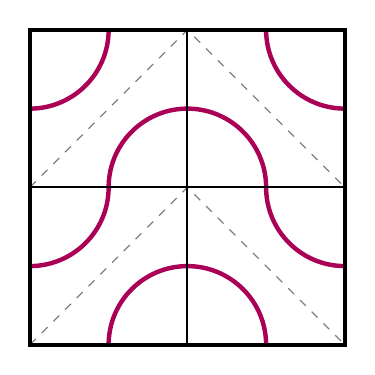
\begin{tikzpicture}[scale=2]
    \draw[ultra thick, draw={rgb:red,2;green,0;blue,1}] 
      (1,0.5) arc (90:180:0.5)  % (0,0)
      (0,0.5) arc (270:360:0.5) % (0,0)
      (1,1.5) arc (90:180:0.5)  % (0,1)
      (0,1.5) arc (270:360:0.5) % (0,1)
      (1.5,0) arc (0:90:0.5)    % (1,0)
      (1.5,1) arc (180:270:0.5) % (1,0)      
      (1.5,1) arc (0:90:0.5)    % (1,1)
      (1.5,2) arc (180:270:0.5) % (1,1)
    ;
    \draw[gray, dashed] (0,0)--(1,1)--(2,0); \draw[gray, dashed] (0,1)--(1,2)--(2,1);
    \draw[ultra thick] (0,0) rectangle (2,2);
    \draw[thick] (1,0)--(1,2) (0,1)--(2,1);
  \end{tikzpicture}\\\vspace{1cm}
  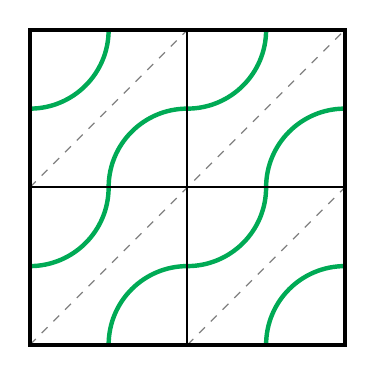
\begin{tikzpicture}[scale=2]
    \draw[ultra thick, draw={rgb:red,0;green,2;blue,1}]
      (2,1.5) arc (90:180:0.5)  % (0,0)
      (1,1.5) arc (270:360:0.5) % (0,0)
      (2,0.5) arc (90:180:0.5)  % (1,0)
      (1,0.5) arc (270:360:0.5) % (1,0)
      (1,1.5) arc (90:180:0.5)  % (0,1)
      (0,1.5) arc (270:360:0.5) % (0,1)
      (1,0.5) arc (90:180:0.5)  % (1,1)
      (0,0.5) arc (270:360:0.5) % (1,1)  
    ;
    \draw[gray, dashed] (0,0)--(1,1)--(2,2); \draw[gray, dashed] (0,1)--(1,2); \draw[gray, dashed] (1,0)--(2,1);
    \draw[ultra thick] (0,0) rectangle (2,2);
    \draw[thick] (1,0)--(1,2) (0,1)--(2,1);
  \end{tikzpicture} \hspace{1cm}
  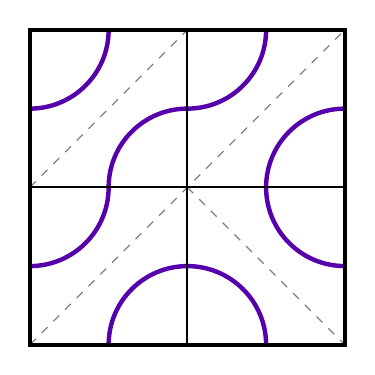
\begin{tikzpicture}[scale=2]
    \draw[ultra thick, draw={rgb:red,1;green,0;blue,2}]
      (2,1.5) arc (90:180:0.5)  % (0,0)
      (1,1.5) arc (270:360:0.5) % (0,0)
      (1.5,0) arc (0:90:0.5)    % (1,0)
      (1.5,1) arc (180:270:0.5) % (1,0)
      (1,1.5) arc (90:180:0.5)  % (0,1)
      (0,1.5) arc (270:360:0.5) % (0,1)
      (1,0.5) arc (90:180:0.5)  % (1,1)
      (0,0.5) arc (270:360:0.5) % (1,1)
    ;
    \draw[gray, dashed] (0,1)--(1,2); \draw[gray, dashed] (0,0)--(1,1)--(2,2); \draw[gray, dashed] (1,1)--(2,0);
    \draw[ultra thick] (0,0) rectangle (2,2);
    \draw[thick] (1,0)--(1,2) (0,1)--(2,1);
  \end{tikzpicture} \hspace{1cm}
  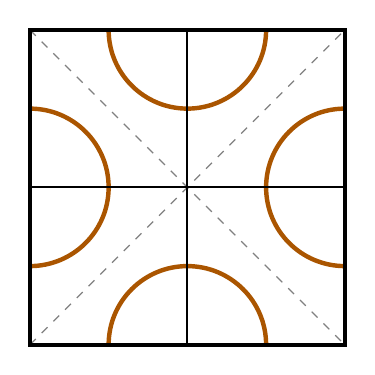
\begin{tikzpicture}[scale=2]
    \draw[ultra thick, draw={rgb:red,2;green,1;blue,0}]
      (1,0.5) arc (90:180:0.5)  % (0,0)
      (0,0.5) arc (270:360:0.5) % (0,0)
      (0.5,1) arc (0:90:0.5)    % (0,1)
      (0.5,2) arc (180:270:0.5) % (0,1)
      (2,1.5) arc (90:180:0.5)  % (1,1)
      (1,1.5) arc (270:360:0.5) % (1,1)
      (1.5,0) arc (0:90:0.5)    % (1,0)
      (1.5,1) arc (180:270:0.5) % (1,0)
    ;
    \draw[gray, dashed] (0,0)--(1,1)--(2,2); \draw[gray, dashed] (0,2)--(1,1)--(2,0);
    \draw[ultra thick] (0,0) rectangle (2,2);
    \draw[thick] (1,0)--(1,2) (0,1)--(2,1);
  \end{tikzpicture}
  \caption {
    An example of the $a(2) = 6$ different ways to fill the $2 \times 2$ grid
    with diagonal tiles (up to dihedral action).
  }
\end{figure}

\begin{question}
  How many such tilings exist?
\end{question}
\begin{related}
  \item What if grids are only counted up to $C_4$ (rotation) action?
  \item What if this is counted on the torus/cylinder/M\"{o}bius strip?
  \item What if each tile can have no diagonals or both diagonals?
  \item What if tiles are black or white?
  \item Is there an obvious bijection between the results on the $2n \times 2n$
    grid for black/white versus diagonal tile types?
\end{related}
\begin{references}
  \item \url{https://oeis.org/A295229}
\end{references}
\end{document}
